\chapter{Company description}
\section{Organizational chart}
Through previous endevors, research and talks with various people which work in different management positions, we've come to this organizational chart. The diagram \ref{fig:organisational-chart} depicts all required departments and their teams as well as management positions. Division are marked with the same color. The color's saturation denotes the hirachical position within said department.

\begin{figure}[!ht]
  \centering
  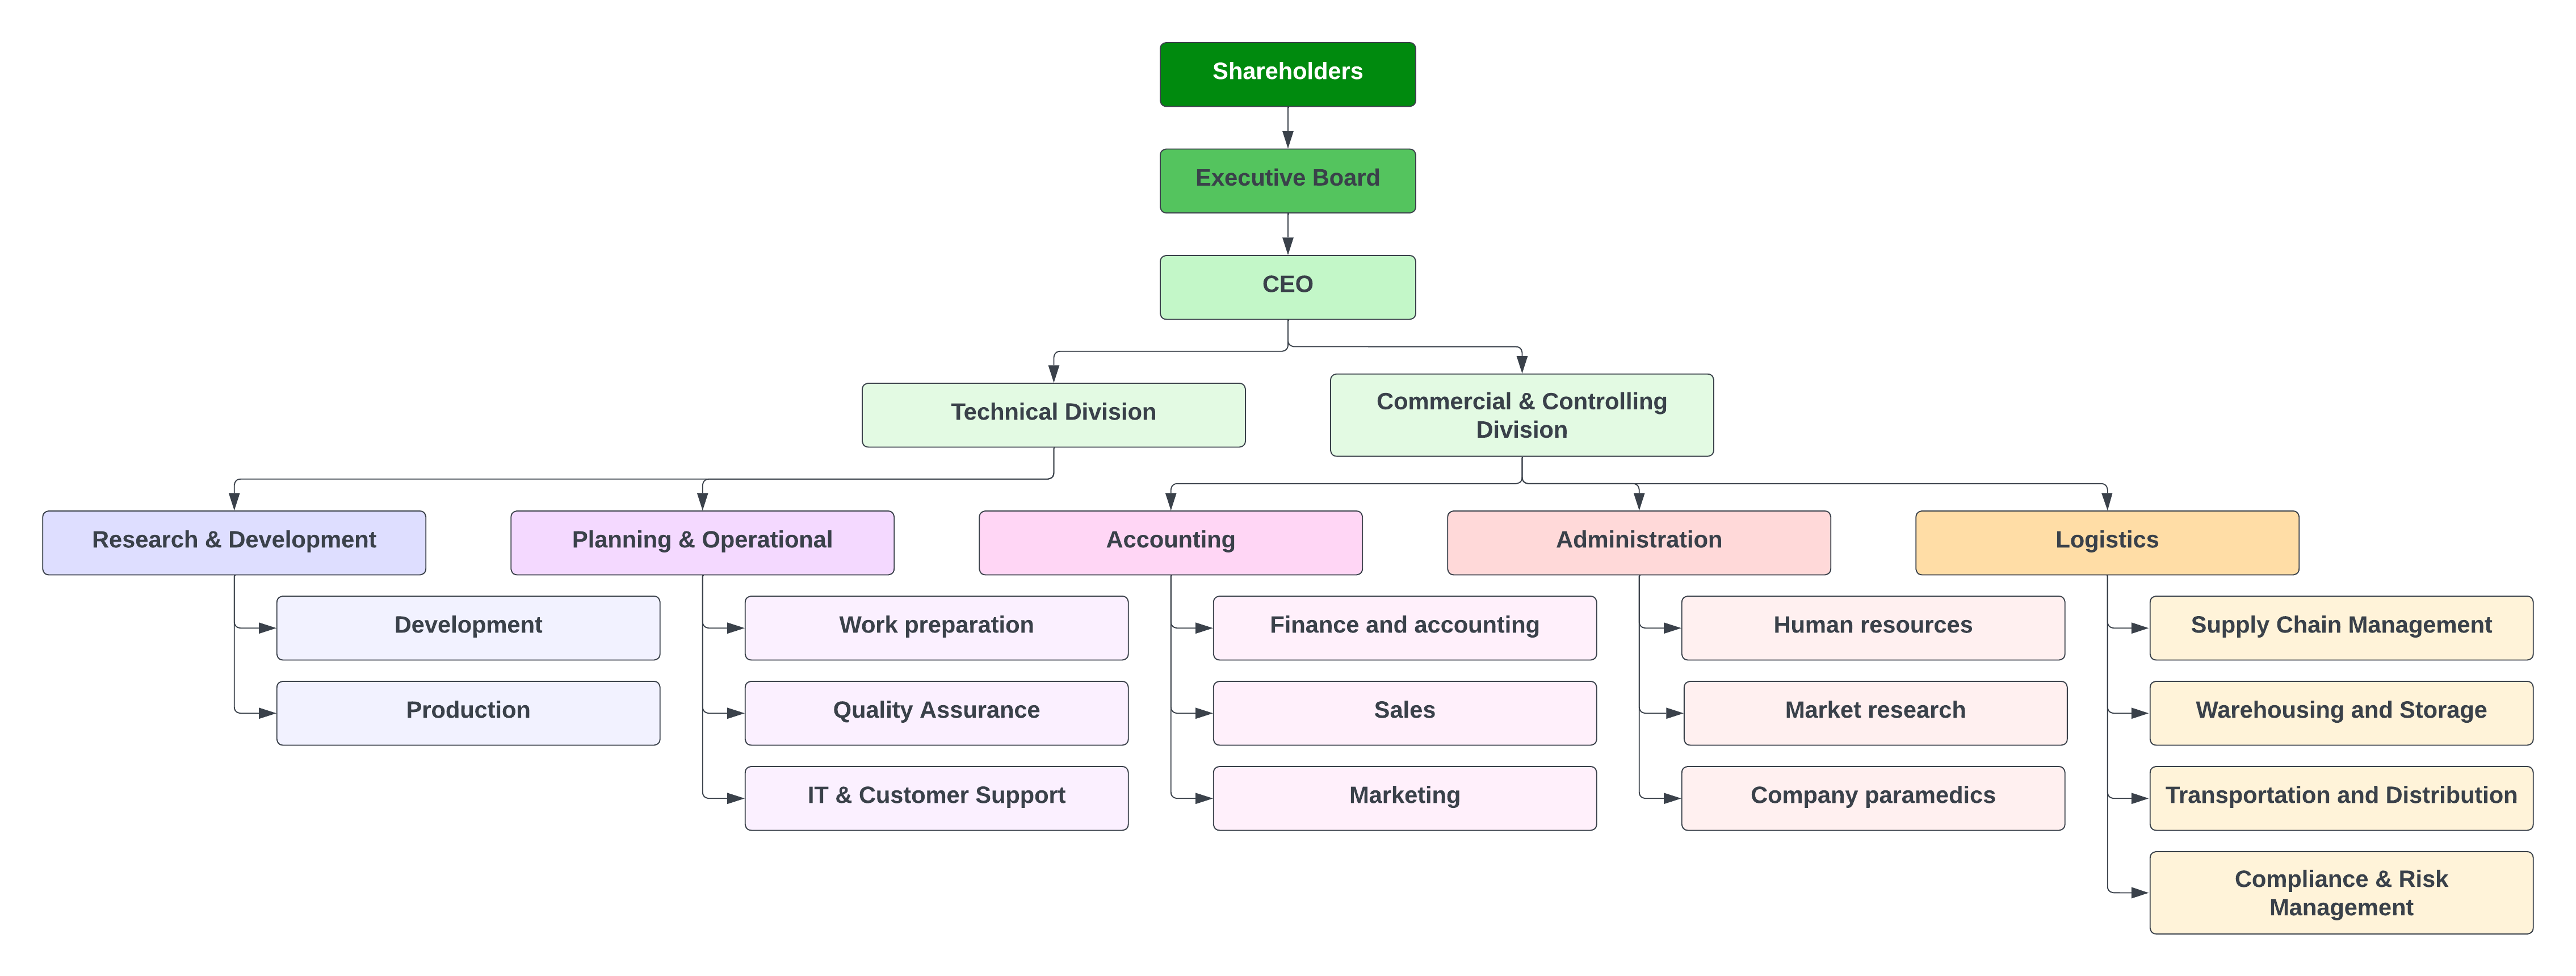
\includegraphics[width=\linewidth]{./images/organisational-chart.png}
  \caption[Organizational chart made with lucidchart.com]{Diagram of the organization}
  \label{fig:organisational-chart}
\end{figure}

This diagram might be more detailed or complex when compared to ones from different startups, but this is by design. It is important that our service works reliably and follows industry standards. To achieve that, we structurally trade a bit of agility for reliability and structure.

Not displayed are ways or means of communication between teams and/or departments. Also, in the future there might be an additional team, which's job is to ignore department barriers and work on different tasks or enable better communication or a better work flow, depending on the workload of a department.

The following chapters \ref{org-management} through \ref{org-logistics} will now go into further detail on what each department entails and of what teams it is made of.
\subsection{Management}\label{org-management}
The management division is marked with the color green.
\subsection{Research \& Development}
\subsection{Planning \& Operational}
\subsection{Accounting}
\subsection{Administration}
\subsection{Logistics}\label{org-logistics}
\section{Vision}
\section{Mission}
\section{Contributions to sustainability}
\section{Objectives of services}
